% Options for packages loaded elsewhere
\PassOptionsToPackage{unicode}{hyperref}
\PassOptionsToPackage{hyphens}{url}
%
\documentclass[
  10pt,
]{article}
\title{World Cup Qatar 2022 predictions: quarter of finals}
\author{Leonardo Egidi, Vasilis Palaskas - Mail:
\href{mailto:legidi@units.it}{\nolinkurl{legidi@units.it}},
\href{mailto:vasilis.palaskas94@gmail.com}{\nolinkurl{vasilis.palaskas94@gmail.com}}}
\date{7 December 2022}

\usepackage{amsmath,amssymb}
\usepackage{lmodern}
\usepackage{iftex}
\ifPDFTeX
  \usepackage[T1]{fontenc}
  \usepackage[utf8]{inputenc}
  \usepackage{textcomp} % provide euro and other symbols
\else % if luatex or xetex
  \usepackage{unicode-math}
  \defaultfontfeatures{Scale=MatchLowercase}
  \defaultfontfeatures[\rmfamily]{Ligatures=TeX,Scale=1}
\fi
% Use upquote if available, for straight quotes in verbatim environments
\IfFileExists{upquote.sty}{\usepackage{upquote}}{}
\IfFileExists{microtype.sty}{% use microtype if available
  \usepackage[]{microtype}
  \UseMicrotypeSet[protrusion]{basicmath} % disable protrusion for tt fonts
}{}
\makeatletter
\@ifundefined{KOMAClassName}{% if non-KOMA class
  \IfFileExists{parskip.sty}{%
    \usepackage{parskip}
  }{% else
    \setlength{\parindent}{0pt}
    \setlength{\parskip}{6pt plus 2pt minus 1pt}}
}{% if KOMA class
  \KOMAoptions{parskip=half}}
\makeatother
\usepackage{xcolor}
\IfFileExists{xurl.sty}{\usepackage{xurl}}{} % add URL line breaks if available
\IfFileExists{bookmark.sty}{\usepackage{bookmark}}{\usepackage{hyperref}}
\hypersetup{
  pdftitle={World Cup Qatar 2022 predictions: quarter of finals},
  pdfauthor={Leonardo Egidi, Vasilis Palaskas - Mail: legidi@units.it, vasilis.palaskas94@gmail.com},
  hidelinks,
  pdfcreator={LaTeX via pandoc}}
\urlstyle{same} % disable monospaced font for URLs
\usepackage[margin=1in]{geometry}
\usepackage{longtable,booktabs,array}
\usepackage{calc} % for calculating minipage widths
% Correct order of tables after \paragraph or \subparagraph
\usepackage{etoolbox}
\makeatletter
\patchcmd\longtable{\par}{\if@noskipsec\mbox{}\fi\par}{}{}
\makeatother
% Allow footnotes in longtable head/foot
\IfFileExists{footnotehyper.sty}{\usepackage{footnotehyper}}{\usepackage{footnote}}
\makesavenoteenv{longtable}
\usepackage{graphicx}
\makeatletter
\def\maxwidth{\ifdim\Gin@nat@width>\linewidth\linewidth\else\Gin@nat@width\fi}
\def\maxheight{\ifdim\Gin@nat@height>\textheight\textheight\else\Gin@nat@height\fi}
\makeatother
% Scale images if necessary, so that they will not overflow the page
% margins by default, and it is still possible to overwrite the defaults
% using explicit options in \includegraphics[width, height, ...]{}
\setkeys{Gin}{width=\maxwidth,height=\maxheight,keepaspectratio}
% Set default figure placement to htbp
\makeatletter
\def\fps@figure{htbp}
\makeatother
\setlength{\emergencystretch}{3em} % prevent overfull lines
\providecommand{\tightlist}{%
  \setlength{\itemsep}{0pt}\setlength{\parskip}{0pt}}
\setcounter{secnumdepth}{-\maxdimen} % remove section numbering
\usepackage{color}
\usepackage{bm}
\ifLuaTeX
  \usepackage{selnolig}  % disable illegal ligatures
\fi

\begin{document}
\maketitle

{
\setcounter{tocdepth}{2}
\tableofcontents
}
\hypertarget{the-statistical-model-in-brief}{%
\section{The statistical model (in
brief)}\label{the-statistical-model-in-brief}}

We use a \textbf{diagonal-inflated Bivariate-Poisson model with dynamic
team-specific abilities} for the attack and the defence. Let
\((X_{i}, Y_{i})\) denote the random number of goals scored by the home
and the away team in the \(i\)-th game, \(i=1,\ldots,n\), respectively.
\(\mathsf{ranking}\) denotes the Coca-Cola FIFA ranking at October 6th,
2022, whereas att and def denote the attack and the defence abilities,
respectively.

\begin{align}
(X_i, Y_i) &\ \sim \ \begin{cases} (1-p) \text{BP}(x_i, y_i |\lambda_1, \lambda_2, \lambda_3) \ \ \ & \text{if} \    x \ne y \\ (1-p) \text{BP}(x_i, y_i | \lambda_1, \lambda_2, \lambda_3) + pD(x, \eta) \ \ \ & \text{if} \   x = y, \end{cases}, \\
\log(\lambda_{1i}) &=\    \text{att}_{h_i, t}+ \text{def}_{a_i,t} + \frac{\gamma}{2}(\mathsf{ranking}_{h_i}-\mathsf{ranking}_{a_i}) \\
\log(\lambda_{2i}) & =\    \text{att}_{a_i,t} + \text{def}_{h_i,t} - \frac{\gamma}{2}(\mathsf{ranking}_{h_i}-\mathsf{ranking}_{a_i}), \ \ i=1,\ldots,n\ (\text{matches}), \\
\log(\lambda_{3i}) & =\ \rho,\\
\text{att}_{k, t}&  \sim \ \mathcal{N}(\text{att}_{k, t-1}, \sigma^2), \\
\text{def}_{k, t} & \sim \  \mathcal{N}(\text{def}_{k, t-1}, \sigma^2),\\
\rho, \ \gamma & \sim \mathcal{N}(0,1) \\
p & \sim \text{Uniform}(0,1)\\
& \sum_{k=1}^{n_t} \text{att}_{k, }=0, \  \sum_{k=1}^{n_t}\text{def}_{k, }=0, \ \ k=1,\ldots n_t \ (\text{teams}), \  t=1,\ldots, T \ (\text{times}).
\label{eq:scoring_rue}
\end{align}

Lines (1) displays the likelihood's equations (diagonal inflated
bivariate Poisson); lines (2)-(4) display the log-linear models for the
scoring rates \(\lambda_{1}, \lambda_{2}\) and the covariance parameter
\(\lambda_3\); lines (5)-(6) display the dynamic prior distributions for
the attack and the defence parameters, respectively; lines (7)-(8)
display prior distributions for the other model parameters; line (9)
displays the sum-to-zero identifiability constraints. Model fitting has
been obtained through the Hamiltonian Monte Carlo sampling, 2000
iterations, 4 chains using the \texttt{footBayes} \texttt{R} package
(with the underlying \texttt{rstan} package). The historical data used
to fit the models come from \emph{all the international matches played
during the years' range 2018-2022 additionally to the group-stage and
the round of 16 matches of World Cup 2022}.

The idea is to provide a dynamic predictive scenario: at the end of each
match-day, the model will be refitted to predict the remaining matches.
Concerning the prediction of matches for the Round of 16 of WC 2022, our
dynamic priors for both the attacking and defensive net abilities of the
competing teams are focused on their previous three matches (group stage
matches of this tournament) in such a way the three previous matches
contribute as a unique temporal period, and not as three distinct
periods. This modification is enabled now since in the last matchday of
the group stages some teams had already qualified to the next phase and
they did not compete with the strongest line-up. Thus, it would be
misleading for our priors to focus more on their last match
performances.

\hypertarget{quarter-of-finals-predictions-9-10-december}{%
\section{Quarter of finals predictions (9-10
December)}\label{quarter-of-finals-predictions-9-10-december}}

Posterior matches probabilities from the posterior predictive
distribution of the model above are displayed in the table below.
\textbf{mlo} denotes the most likely exact outcome (in parenthesis, the
corresponding posterior probability). Darker regions in the plots below
denote more likely outcomes: on the \(x\)-axis the favorite team goals, on the
\(y\)-axis the underdog team goals.

\begin{longtable}[]{@{}llcccc@{}}
\toprule
favorite & underdog & fav. win & draw & und. win & mlo \\
\midrule
\endhead
Brazil & Croatia   &0.676  & 0.220 & 0.104 & 1-0 (0.16) \\
Argentina & Netherlands   & 0.414 &  0.264 & 0.322   & 0-0 (0.172) \\
Portugal & Morocco & 0.536  & 0.191 & 0.273   & 1-0 (0.16) \\
England & France & 0.361 & 0.292 & 0.348 & 0-0 (0.126) \\
\bottomrule
\end{longtable}

\begin{center}\rule{0.5\linewidth}{0.5pt}\end{center}

\begin{center}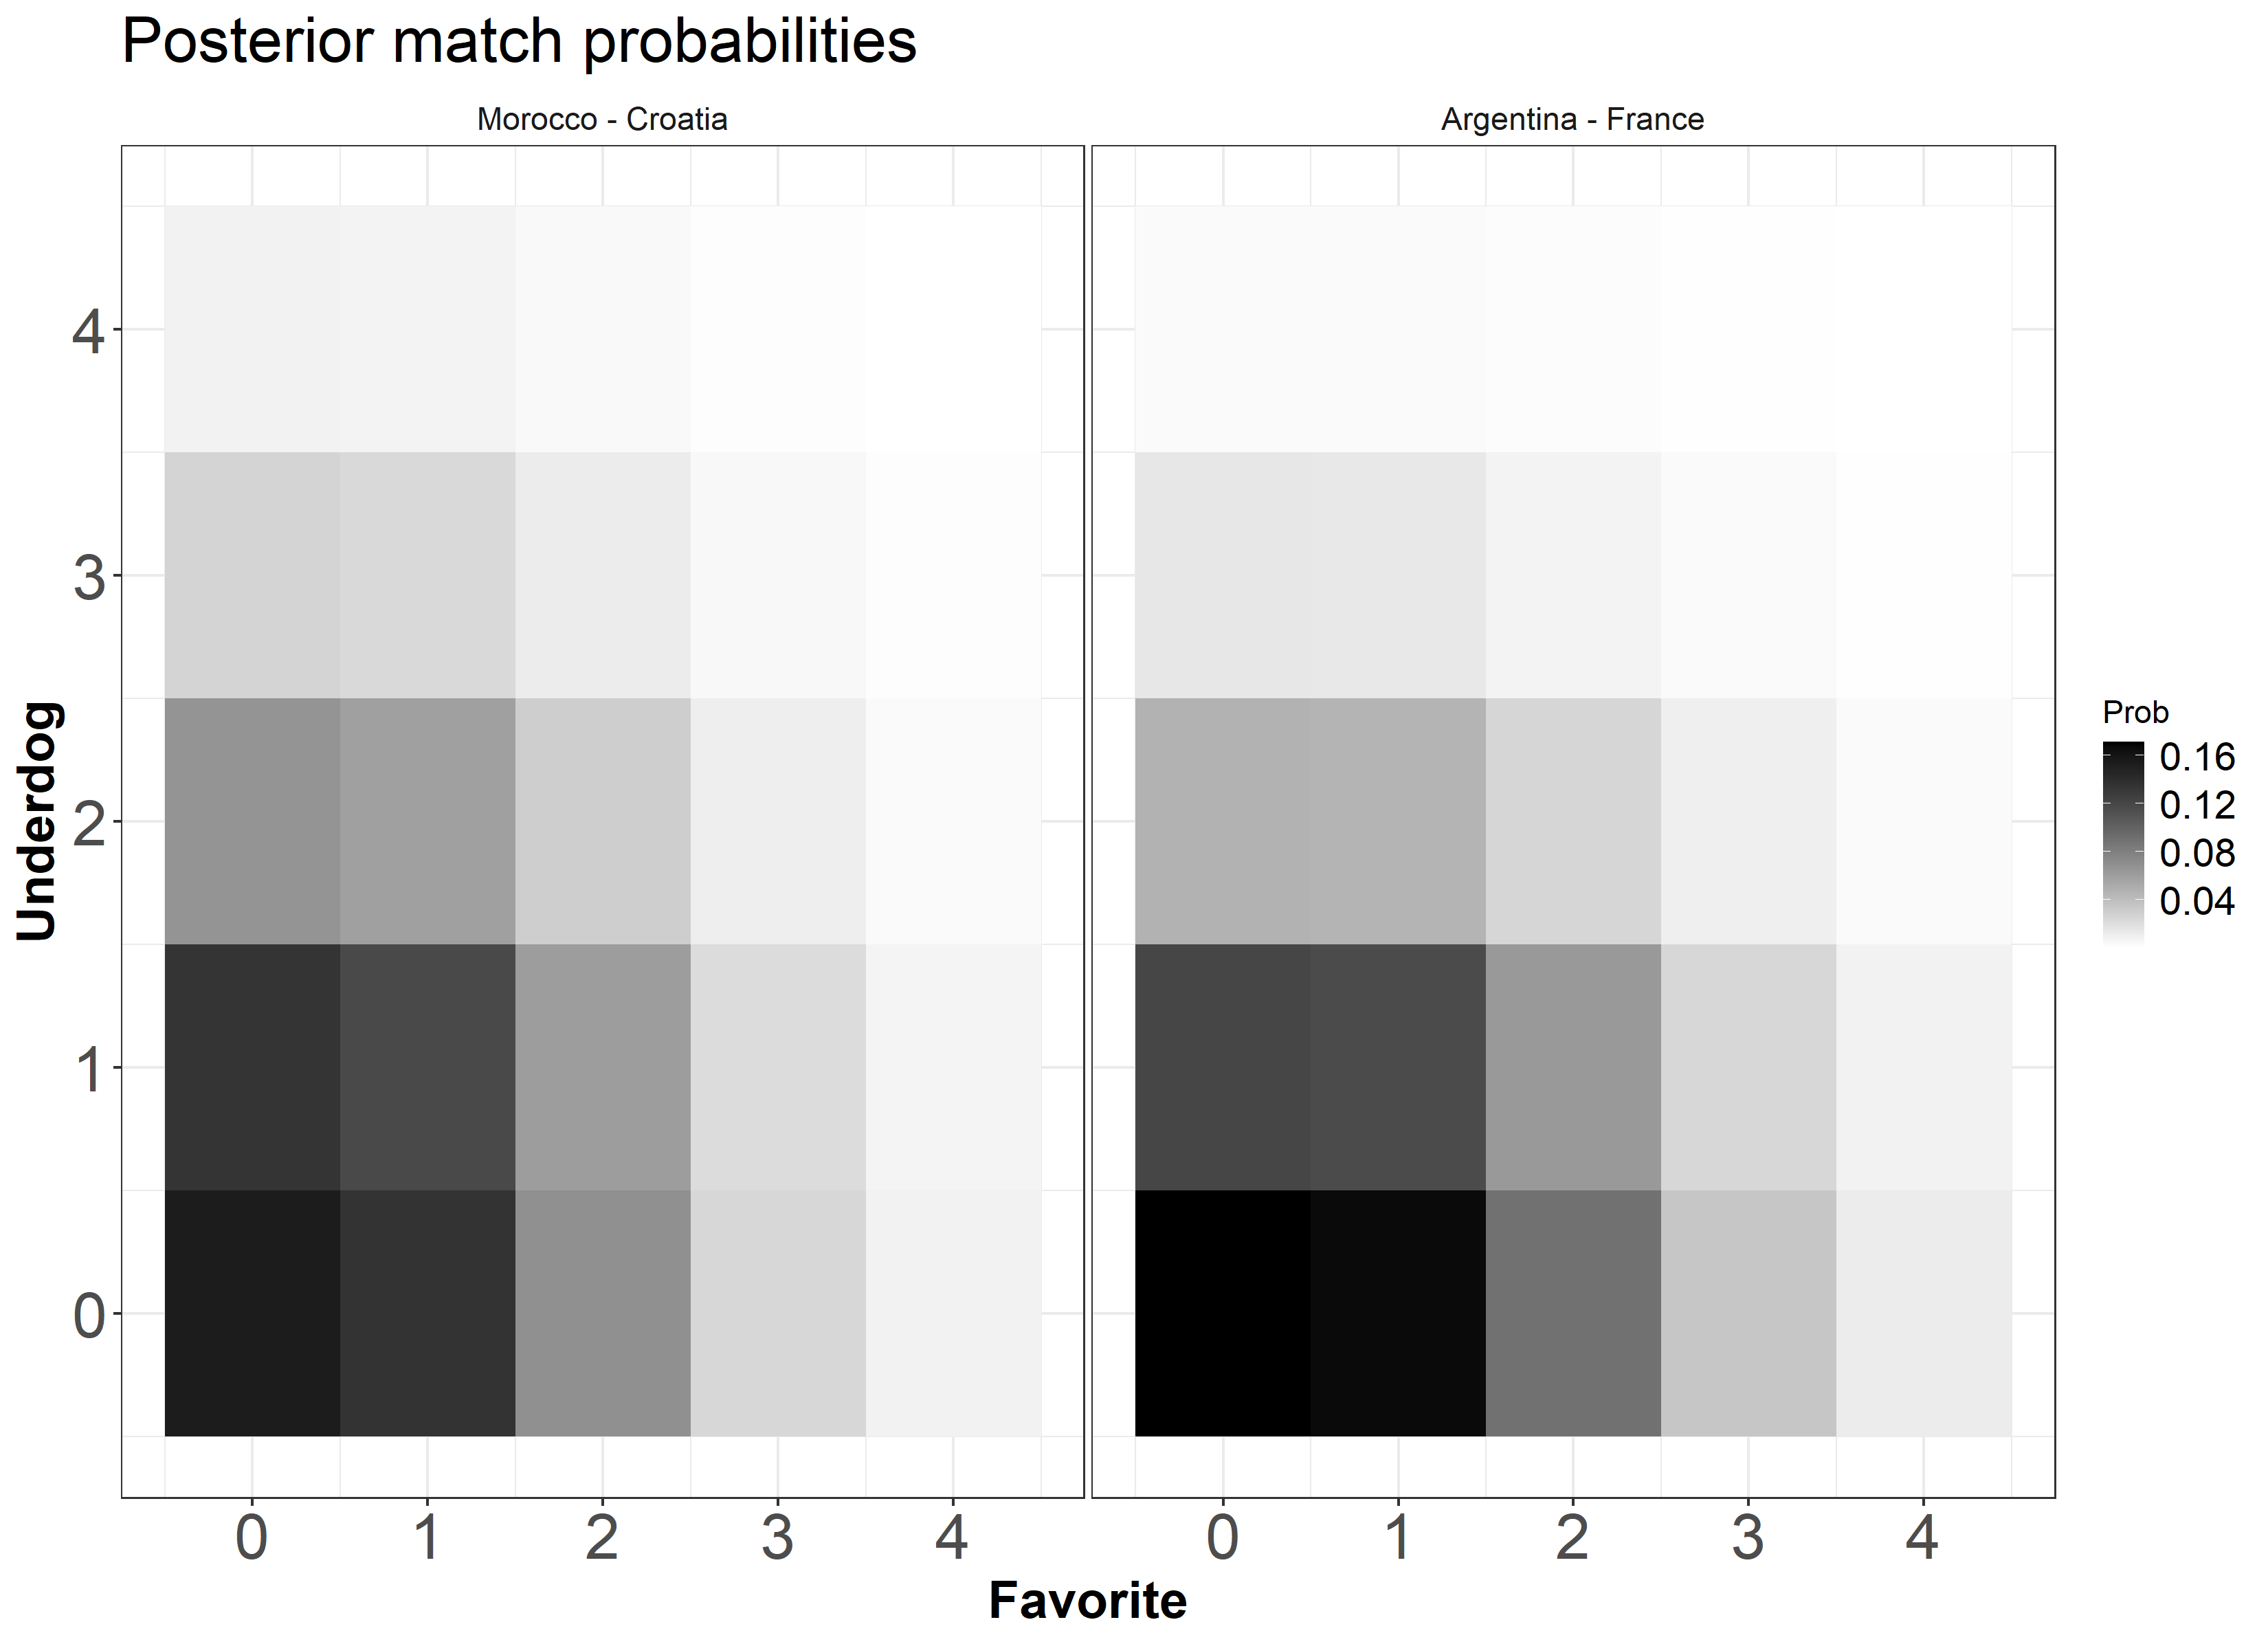
\includegraphics[width=0.8\linewidth]{figs/data2-1} \end{center}


\section{Predictive performance results}

In this section, we considered to evaluate the predictive performance of some proposed models, focused on the goals scored by both competing teams, across matchdays held until the end of phase 16 of the tournament ($n=56$ matches). The models which were compared among each other:

\begin{enumerate}
\item Diagonal Inflated Bivariate Poisson
\item Bivariate Poisson
\item Double Poisson
\end{enumerate}

For the fitting of all these models, we used the same data for their training as well as the same priors apart from both formulations of bivariate Poisson (models 1 and 2) where we had the additional parameters of $\pi, \rho$ for model 1 and the one of parameter $\rho$ for model 2, respectively. The dataset for the performance evaluation consists of 56 matches.

Predictive Performance Results:
First, we calculated the Bayesian Information Criterion of LOOIC (Vehtari et al., 2017) across Models 1, 2, 3 in every matchday of this period. Briefly, we report that the LOOIC of the Model 1 was the worst one in every match day while the best one was the third one but with much slight difference compared to the model 2.
As a next step, we considered to compare our fitted models’ predictive performance, using the posterior predictive density of goal difference, with the observed goal differences. More specifically, we proceeded to the comparison of our posterior predictive distributions (of fitted models) with the observed goal differences graphically through the posterior predictive checking (PPC) bar plots. These plots are useful since we can depict how close are the 95\% posterior intervals of the predicted frequencies of goal differences to the corresponding observed ones. Also, the plots will include the metric of “Mean Absolute Error” calculated within Bayesian framework to quantify how close are our model-based predictions with the observed results across the group stage matches.  Based on Figure 1, we observe that all fitted models present similar performance in terms of both graphical representation and the error metric of MAE. The similarity between predictive performances of all fitted models is obvious from the corresponding PPC graphs where in all those ones, the posterior medians (dark points) are close to the observed frequencies. An obvious difference between fitted models is that the Model 1 predicts with inflation the draw match outcome (goal difference equal to zero) compared to the Models 2 and 3 which is reasonable due to its own model formulation using the inflation parameter of p. 


\begin{center}
\begin{figure}
 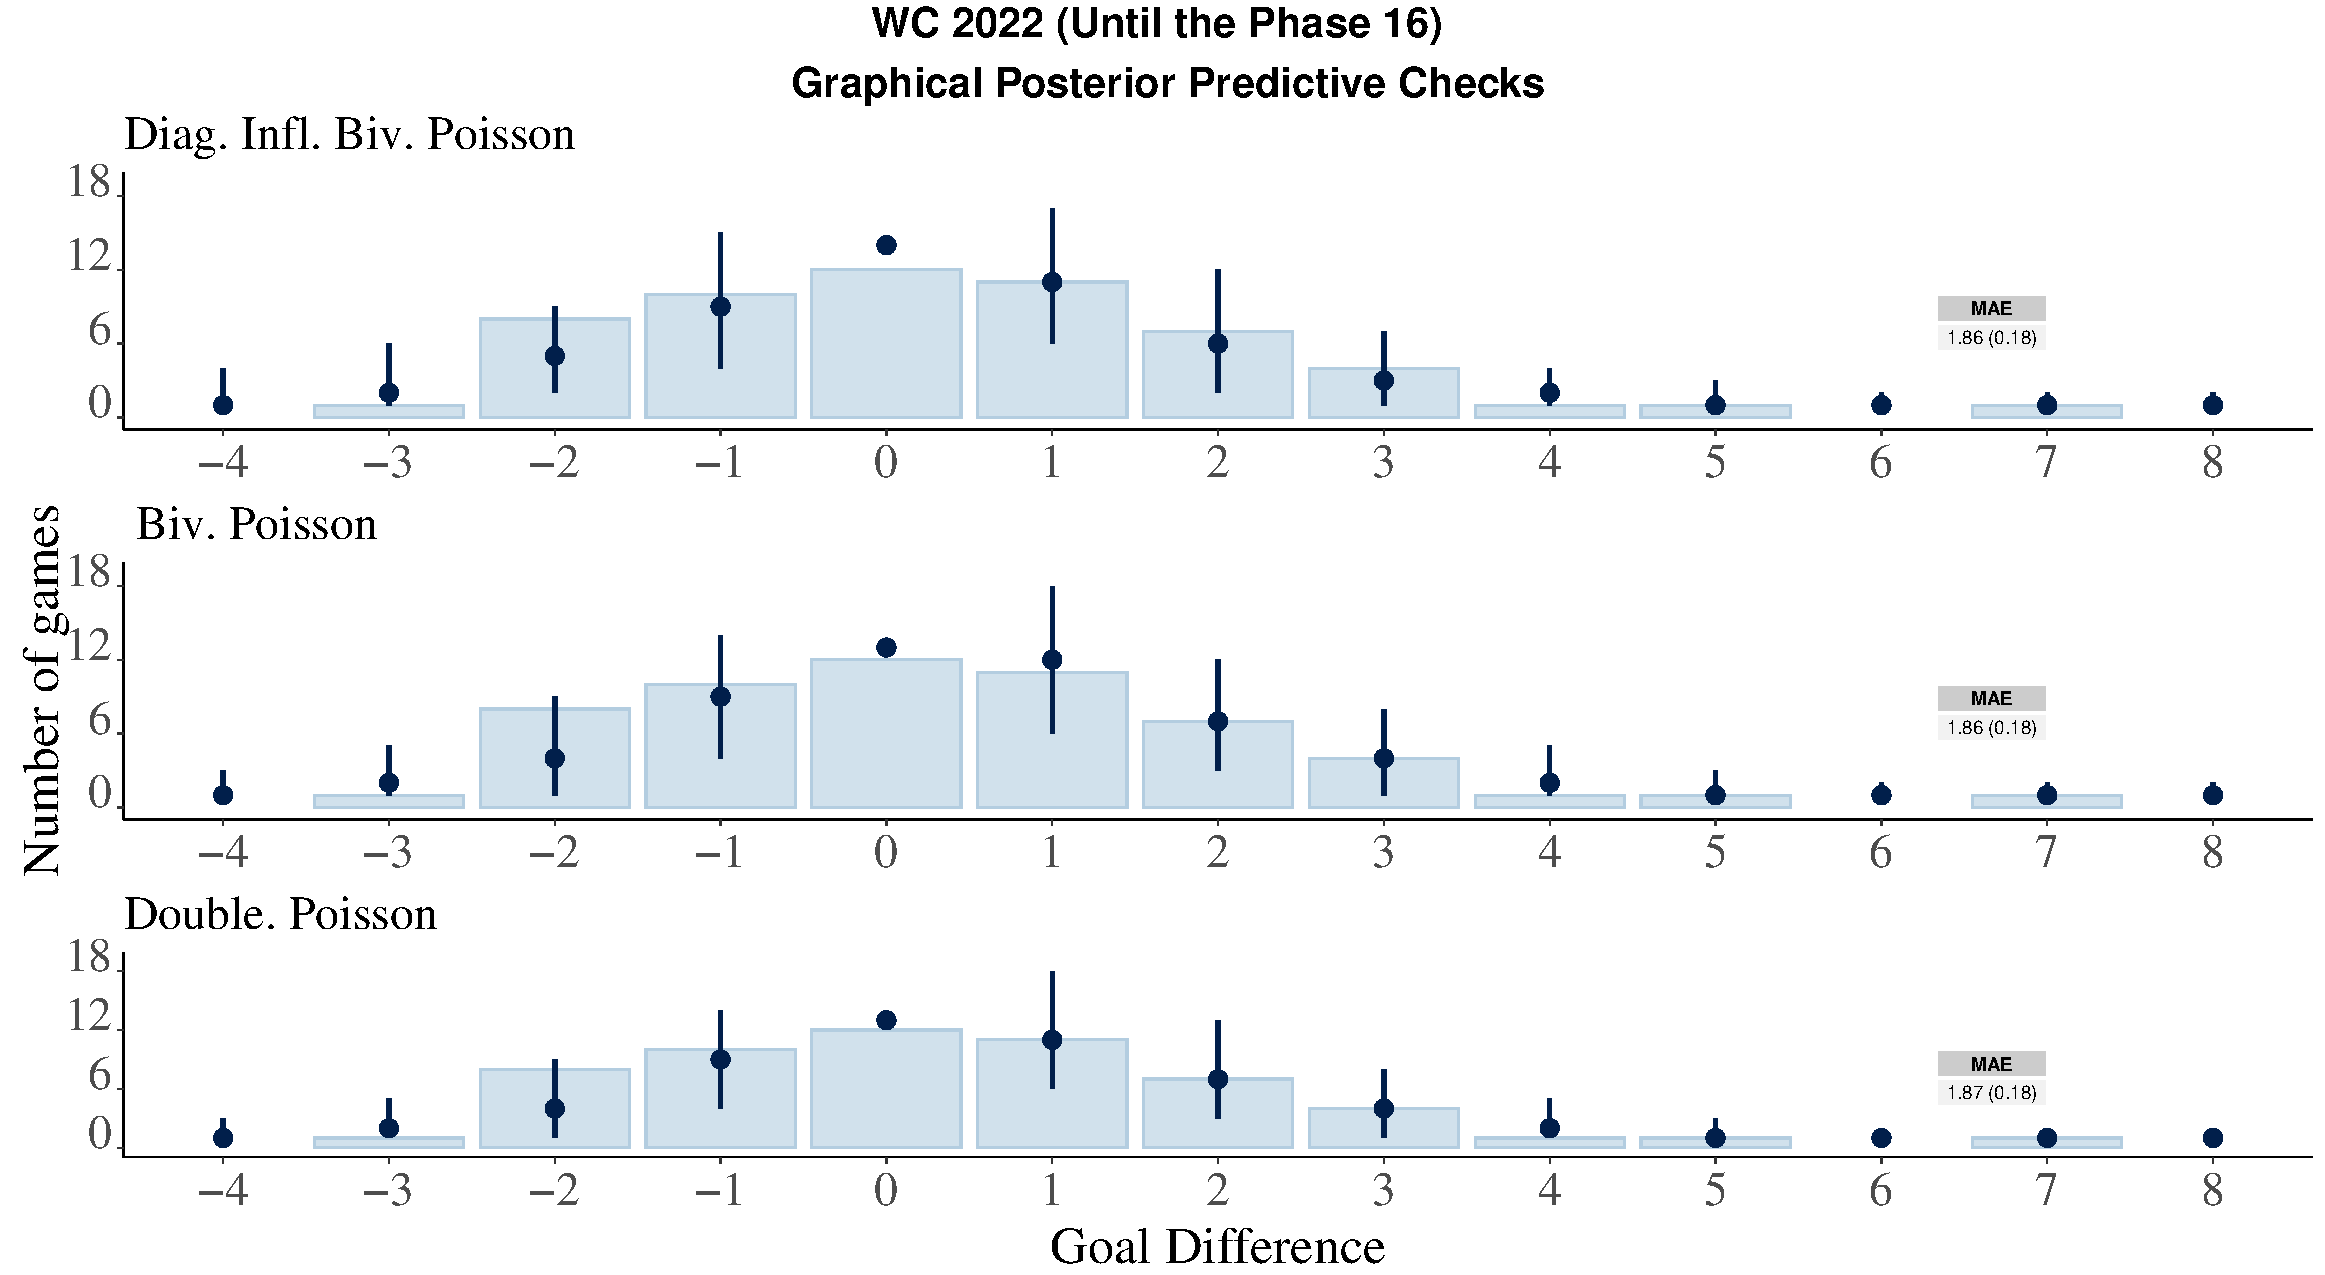
\includegraphics[width=0.8\linewidth]{WC_2022_Out_Sample_PPC.pdf}
\caption{95\% Posterior intervals of predicted frequencies of goal differences; Blue dark points and blue bars are the generated posterior predictive distribution median and the observed quantities (frequencies), respectively. The MAE metric is the posterior mean of the MAE; within brackets the posterior standard deviation of this metric} 
 \end{figure}
  \end{center}

\begin{center}
\begin{figure} 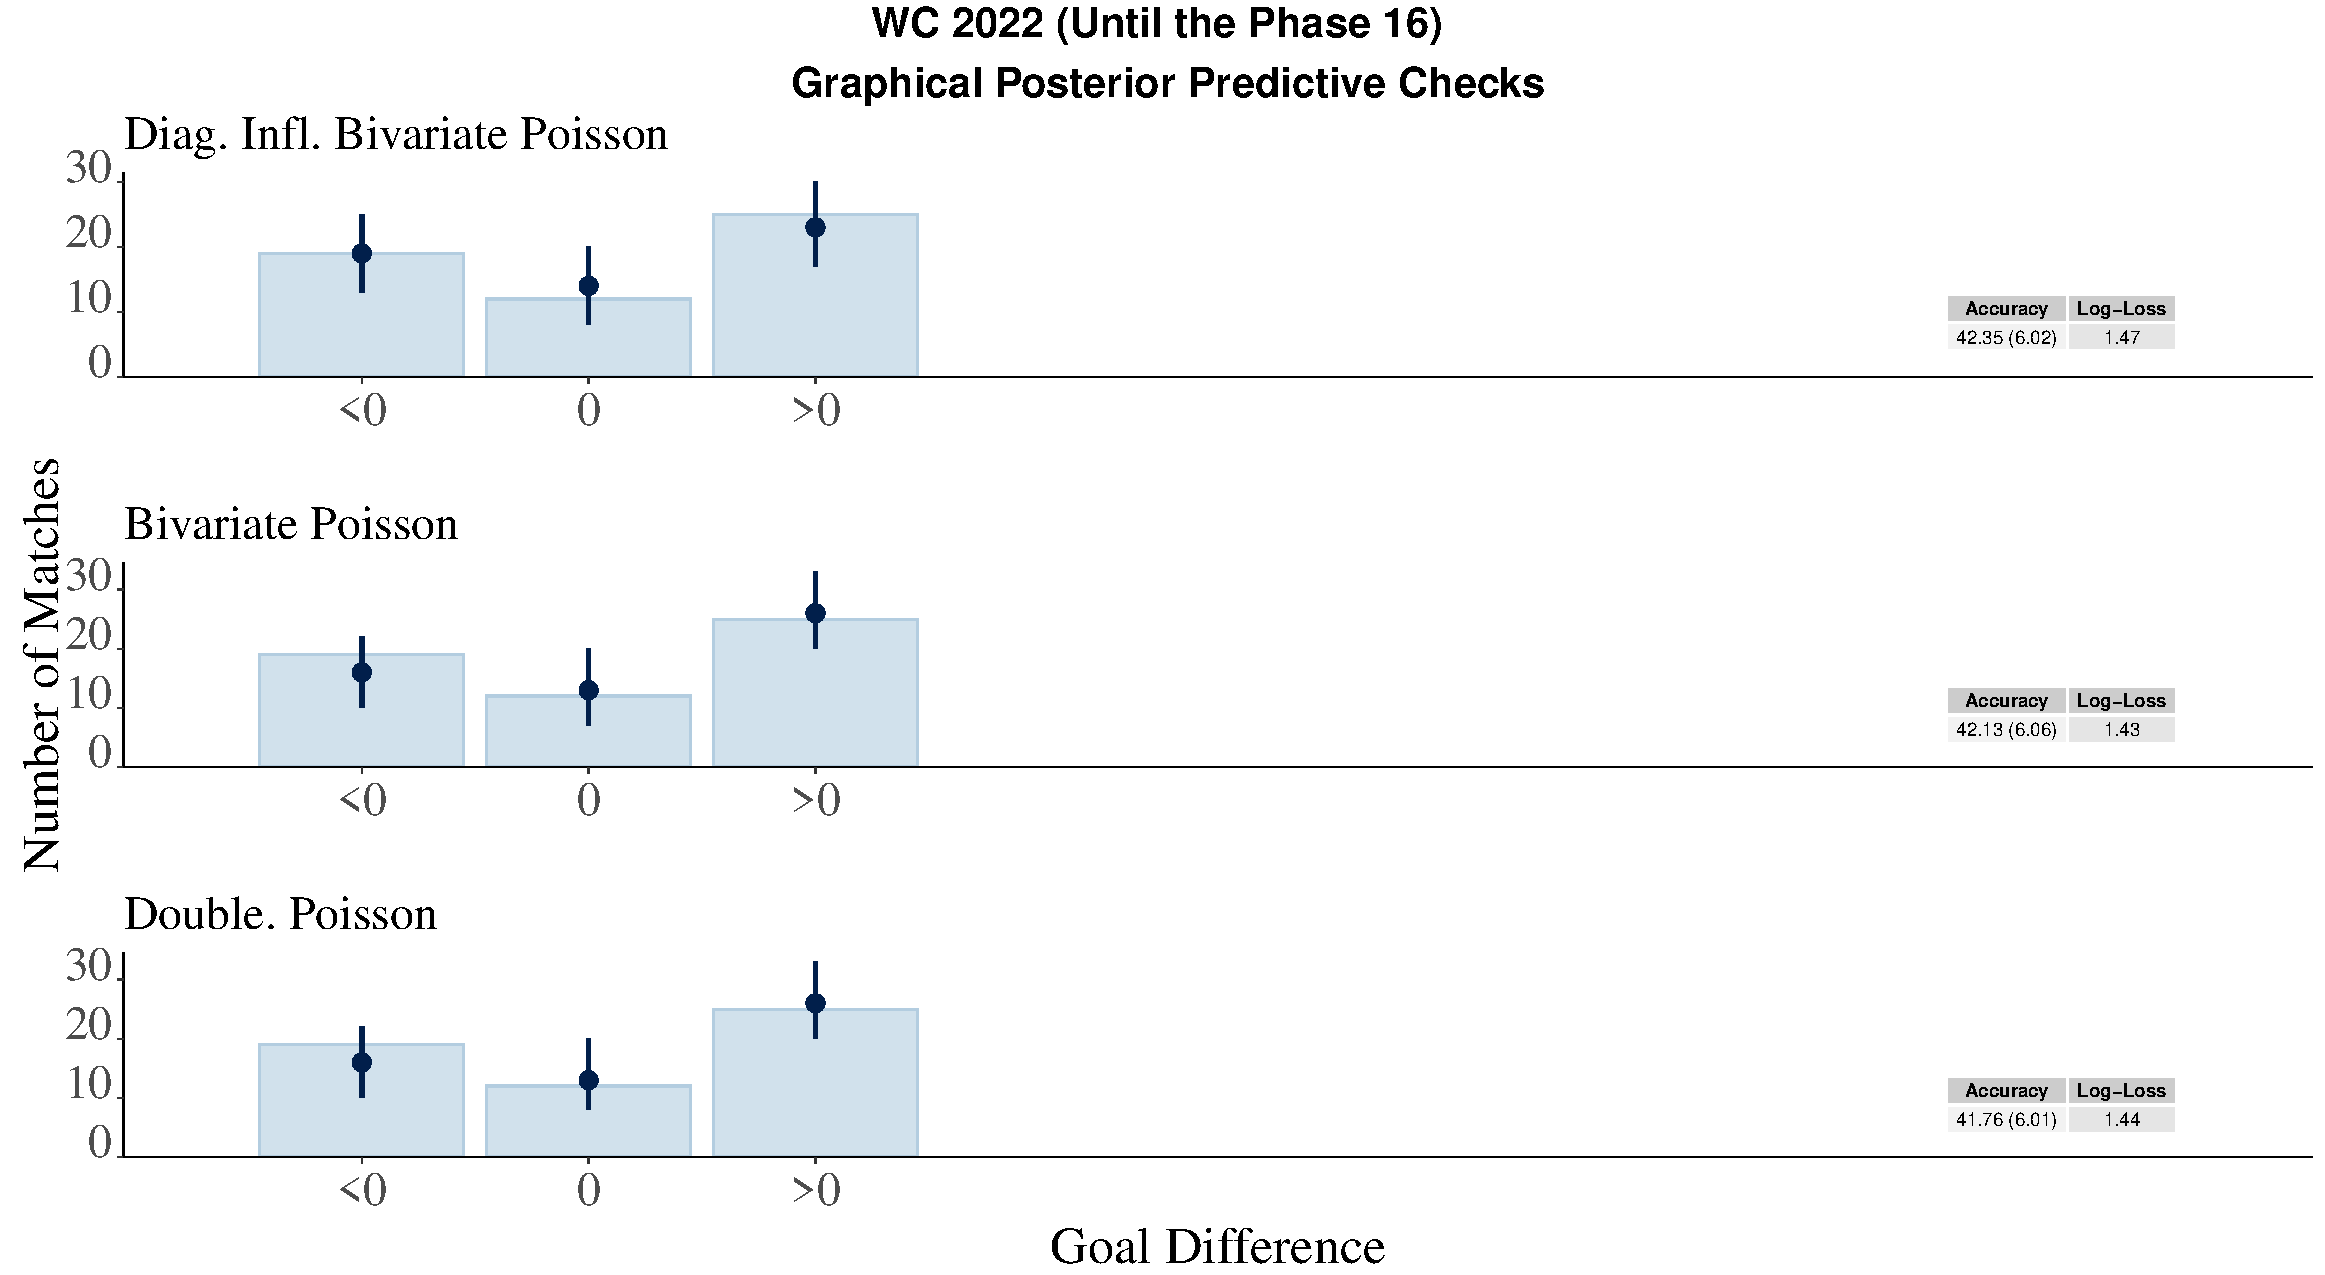
\includegraphics[width=0.8\linewidth]{WC_2022_Out_Sample_PPC_Classification.pdf}
\caption{95\% Posterior intervals of predicted frequencies of goal differences reflecting the three-way match outcome (win of home team, draw, win of the away team); Blue dark points and blue bars are the generated posterior predictive distribution median and the observed quantities (frequencies), respectively. The accuracy metric is the posterior mean of the MAE; within brackets the posterior standard deviation of this metric.}
\end{figure}
\end{center}



In general, the results from Figure 1 indicate that any model among them provides similar predictions with a little advantage in favor of both models 1 and 2. For this reason, we proceeded to an additional check to identify potential predictive performance differences between of the Models 1-2.  

More specifically, the mixed results of LOO and MAE led us to compare our models based on their predictive performance only on the final match outcome without considering the exact goal difference of the teams. Since now our interest is focused on three possible outcomes (home team win, draw, away team win), our predictive performance results will be based on both the accuracy and the multi-class log loss (multi-class cross entropy; for more details about this metric see Grandini, M., et. al, 2020). The multi-class log loss metric is more appropriate for such classification tasks since our problem are not yet perfectly balanced and it is an evaluation metric quantifying how close are our probabilistic predictions with the observed final match outcomes. However, the results of both metrics are presented in Figure 2 with the corresponding PPC plot. In contrast with Figure 1, here the evaluation metrics suggest that the simple form of Bivariate Poisson (i.e., Model 2) is slightly better from Model 1 in terms of predictive performance.  


In conclusion, our predictions for the remaining matches of the World Cup will be now based on the Model 2 (Bivariate Poisson). The specific change in our modelling strategy is based on the following reasons:
\begin{itemize}
\item	LOO-IC was much lower in Model 2 compared to the Model 1.
\item Due to the consistency of MAE and PPC results for the original scale of the goal difference response variable, both accuracy and multi-class log-loss indicated as better modelling option the second one.
\item The simple Bivariate Poisson is simpler in fitting than the Model 1 in terms of parameter space complexity (Model 1 includes additional the parameter of inflation.
\end{itemize}

 Nevertheless, an external reader can obtain similar results in terms of error metrics by fitting any choice among first two models to predict the goals scored by two competing teams as well as the goal difference in each match.

By the end of tournament, as we will obtain more and more matches to our sample, we are going to proceed a more detailed evaluation of the predictive performance of fitted models by using additional error metrics such as log-loss metrics, another classification metrics such as AUC, F1, etc.… to understand at great extent which model would perform better to such tournament based on the training data that we use for.

\emph{We'll use bivariate Poisson model for semifinals and finals.}




\end{document}
